\section[Historia]{Historia języka androyasańskiego}

\begin{spacing}{1.1}
Na planecie Maŕid, na której znajduje się Cesarstwo And́royas istnieje szereg 
głównych rodzin językowych: języki nenneckie (staronennecki, doryński, 
androyasański cesarski), języki turańskie (agaveński, turański, chicha), język 
papityjski (izolowany), języki nagiryjsie (nagiryjski, almefig, alnogh), 
języki wschodnie (maddyjski, woymnarski), języki mistralskie (fetucki, zapański, 
tebajski, zou, mistralski), języki kaireńskie (lono, kaireński, starolamecki, 
lamecki), języki chi\-zelsko-keilijskie (chizelski, keilijski, esrański), języki 
nahadyjskie (rilla, nahadyjski).

Najwcześniejsze zabytki językowe, które udało się odkryć, to pismo kahejskie na 
glinianych tablicach sprzed około 5000 lat przed Zjednoczeniem.

Język androyasański (\emph{Inrat yi Androias}), początkowo znany był jako 
androyasański cesarski lub po prostu cesarski (\emph{eygepa inrat}), 
najpowszechniej nazywany jest po prostu \emph{andro} i~jest językiem częściowo 
sztucznym. Powstał na podstawie języka handlarzy używanego w~kontaktach pomiędzy 
Królestwem Nennek, a~krajami Zachodu i~został zaproponowany jako drugorzędny 
język urzędowy po powstaniu Drugiego Cesarstwa. Łącząc cechy języka 
staronenneckiego, kaireńskiego, keilijskiego i~turańskiego wydawał się idealnym 
kandydatem na język zjednoczonych krajów.

Androyasański cesarski był krytykowany ze względu na istnienie tam bardzo 
silnego związku z~językiem nenneckim, co powodowało pewne trudności: na przykład 
w~zapisie w~sylabicznym piśmie chizelskim. Jednak po upadku Drugiego Cesarstwa 
już był rozpowszechniony jako język warstw wyższych i~stawał się narzędziem 
uniwersalnej komunikacji, a~potem ewoluował jak każdy język naturalny.

Jedną z~bardziej istotnych zmian w~historii języka andro jest przejście z~języka
cesarskiego do współczesnego andro, w~której między innymi utrata formy czasu
przyszłego na rzecz partykuły \emph{ze}, zmiana formy użycia partykuł \emph{do}
oraz \emph{hemi}, utrata głoski [y] i~podobne.

Od powstania Trzeciego Cesarstwa, a~także poprzez wpływ Cesarstwa, jest jedynym 
językiem, który jest znany na wszystkich Wyspach i~jest nauczany we wszystkich 
krajach, włączając z~w to Wolne Stany Ezimruk. Począwszy od początku XX wieku, 
Republika Nennek nie uczy już powszechnie języka nenneckiego w~szkołach, 
zastąpiwszy go tylko i~wyłącznie androyasańskim oraz turańskim.

Do zapisu języka używa się dwóch sposobów --  ideograficzno-sylabicznego,
tzw. nowoczesnego (\emph{nu͞er isdara͞o huark} -- dosłownie
,,nowe podzielone słowa'') oraz alfabetu fonetycznego -- \emph{chiwo}.

Alfabet fonetyczny ma 27 liter i nie rozróżnia liter wielkości znaków, sylabariusz 
ma 24 znaki podstawowe z których składa się około 70 znaków sylabicznych; 
ma również kilkadziesiąt znaków ideograficznych. W latach 1800-1817 przeprowadzona
została reforma systemu sylabicznego, w~którym ustalono nowe, prostsze reguły zapisu.

Pismo fonetyczne, w wersji odręcznej, może wyglądać w następujący sposób:

\begin{center}
    
\includegraphics[width=5cm]{katia-signature.png}    
\end{center}

Jest to odręczny zapis imienia \emph{Katia}, ręką samej cesarzowej, \textbf{Katii mal Arkai}.
Jej mąż, \textbf{So'tak mal Valor}, podpisuje się następująco:

\begin{center}
    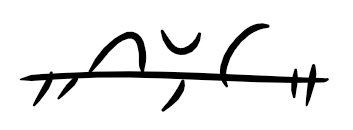
\includegraphics[width=5cm]{sotak.png}
\end{center}

Zapis w alfabecie fonetycznym, z wykorzystaniem specjalnego kroju \emph{desaho},
przeznaczonego do pisania znaków drogowych, informacji turystycznej i innych
informacji publicznych wygląda następująco:

\begin{center}
    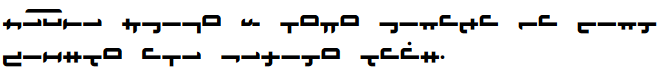
\includegraphics[width=12cm]{desaho.png}
\end{center}

\note{Tekst ten, \emph{ze͞uye chido yi boso hinaja va fint wirklo abe gepito laák}
nie ma większego sensu, ale jest to pangram -- używany jako odpowiednik polskiego
,,pchnąć w tę łódź jeża lub ośm skrzyń fig''.}
\skipline

W 2007 roku zaproponowana została transkrypcja androyasańskiego do alfabetu 
łacińskiego (transkrypcja Kadala), poprawiona w~latach 2013-2014 (transkrypcja 
Ziri). W~tym słowniku używana jest tylko i wyłącznie transkrypcja Ziri.

Język nie jest całkowicie jednorodny -- jako, że włada nim ponad miliard 
użytkowników, pojawiają się w~nim dialekty oraz zachowania i~zasady specyficzne 
dla danej kultury lub regionu. 

Obecnie wyróżnia się 6 głównych dialektów: 

\begin{itemize}
    \item dialekt nennecki, wyróżnia się brakiem stosowania zaimków egli/egla oraz formalnych epié/epiá,
    \item dialekt zachodni, w~którym preferowany jest przyrostek dzierżawczy <-yi> zamiast partykuły \emph{yi},
    \item dialekt północny wyróżniający się pojawianiem się fonemu /ʃ/ zamiast /ʐ/,
    \item dialekt pustynny,
    \item dialekt południowo-wschodni.
\end{itemize}

Ten słownik skupiać się będzie na literackiej formie języka androyasańskiego, 
nazywanej czasami \emph{ardo andro} (wysoki androyasański), pewne uwagi 
dotyczące dialektów będą zawarte w~dodatkowych opisach do haseł.

\end{spacing}